\section{Deterministic State Generator}

\subsection{Methodology}

As the hardware limitations prevent the creation of complete system models, a smaller subset was utilised for analysis. All systems were created with the following parameters (parameters were inflated to accelerate the decay of reward valuation):

\begin{itemize}
    \item Blockchain 
    \begin{itemize}
        \item Block reward - 1
    \end{itemize}  
    \item Pool 
    \begin{itemize}
        \item Initial chunks - 2
    \end{itemize}
    \item Participants
    \begin{itemize}
        \item Initial funds - 1
        \item Initial chunks - 0
    \end{itemize}
    \item Reward minimum threshold - 0.009
    \item Maximum depth - 15
\end{itemize}

The following metrics were recorded regarding each participants potential expected reward based on different participation chances.

\begin{itemize}
    \item The most equal state (smallest difference in balance).
    \item The least equal state (greatest difference in balance).
    \item Total end states.
    \item Total end states within the given wealth-difference.
    \item Metrics for each participant which includes:
    \begin{itemize}
        \item The number of states reachable with the highest balance.
        \item The highest balance possible.
        \item The number of states reachable with the lowest balance.
        \item The lowest balance possible.
        \item The total number of states within the given wealth-difference.
    \end{itemize}
\end{itemize}

\subsection{Results}

Even before generating any states, some intuitive assumptions can be made regarding the potential outcomes of a game in which only two participants exist:

\begin{itemize}
    \item If both participants purchase from the pool in the first step and continue to purchase from each other or do not purchase at all in consequent steps, they will always be in  equilibrium (i.e. equal balance).
    \item The highest possible balance achievable while in equilibrium is if both participants hold a chunk each and do not purchase.
    \item The results will be symmetric for participants (unless probability or initial state is different).
\end{itemize}

Consider a game in which the initial state is as follows.

\begin{itemize}
    \item Pool - chunks: 2, balance: 0
    \item Participant 1 - chunks: 0, balance: 1
    \item Participant 2 - chunks: 0, balance: 1
\end{itemize}

The expected payout for all action combinations can be seen in \cref{table:payout1} below. 

\begin{table}[H]
  \centering
  \caption{Expected payout for a basic two-player game}
  \label{table:payout1}
  \begin{tabular}{|l||*{5}{c|}}\hline
    \backslashbox{Participant 1}{Participant 2} & \makebox{Skip} & \makebox{Purchase} \\
    \hline \hline
    Skip                                        & 0, 0           & 0, 1 \\ \hline
    Purchase                                    & 1, 0           & 2, 2 \\ \hline
  \end{tabular}
\end{table}

In the case where both participants skip (Skip, Skip), they receive no rewards (having no chunks). If both participants purchase at the same time (Purchase, Purchase), they expend their balance in order to buy the chunk from their opponent and receive an equal amount of funds for selling their chunk to their opponent, resulting in no net change in balance. Then, during the reward phase, both participants receive one unit for having one chunk in their possession. In cases where only one participant purchases (Skip, Purchase), only the purchaser expends their balance but does not receive any as a chunk was not purchased from them. Next, they receive a reward, restoring their balance back to 1. In this case, the participant who opted to skip would consider purchasing a chunk to catch up, returning to the action combination (Purchase, Purchase). Hence, there exists a Nash equilibrium with the action combination (Purchase, Purchase).

A test was run using the generator for participant probabilities ranging from 0.1 to 0.9 for both participants with a tax rate of 0 and 0.2 (the test script can be found in \cref{appendix:testparticipationprobability}). Only one participant is considered as they are symmetrical in all aspects.

\begin{figure}[H]
  \centering
  \caption{Expected reward per combination of participant purchase probability}
  \label{figure:state-expected}
  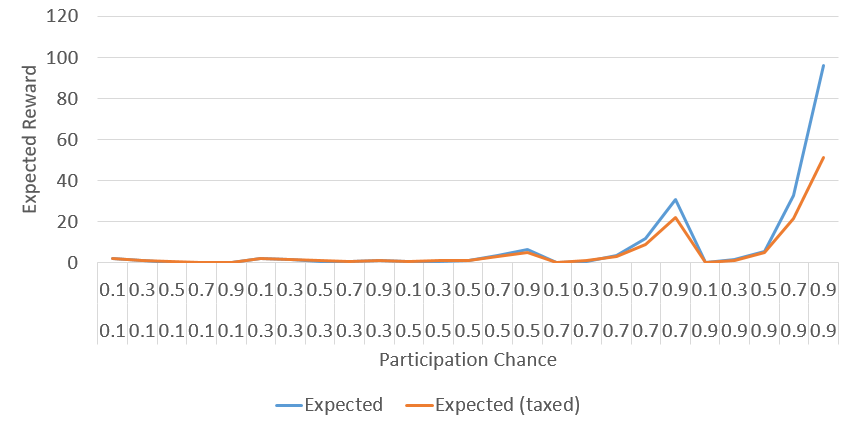
\includegraphics[width=\textwidth]{media/state-expected.PNG}
\end{figure}

The results seen in \cref{figure:state-expected} above shows the expected reward per combination of participation chances. Participant 1 on the bottom row and participant 2 on the top row. It can be observed that higher participation rates yield a higher expected reward, with spikes each time both participation chances reach a relatively high value. This is likely due to the fact that as the product of the probabilities yields the maximum possible chance a state may achieve, reducing the expected reward accordingly. For example, given participants 1 and 2 both have a 0.1 chance to participate, the combination is $0.1 \times 0.1 = 0.01$, meaning the final reward is reduced by x100. Similarly, given participants 1 and 2 both have 0.9 chance to participate, the combination $0.9 \times 0.9 = 0.81$ is significantly higher with at most a 19\% reduction. It is also noted that the impact of the tax becomes more pronounced as the probability to purchase increases. This is likely due to participants being taxed more frequently as they are more likely to possess chunks given the higher purchase probability.

Figure \ref{figure:state-bestworst} below shows the probability of reaching the states with the highest and lowest balance.

\begin{figure}[H]
  \centering
  \caption{Probability of reaching state with highest and lowest balance}
  \label{figure:state-bestworst}
  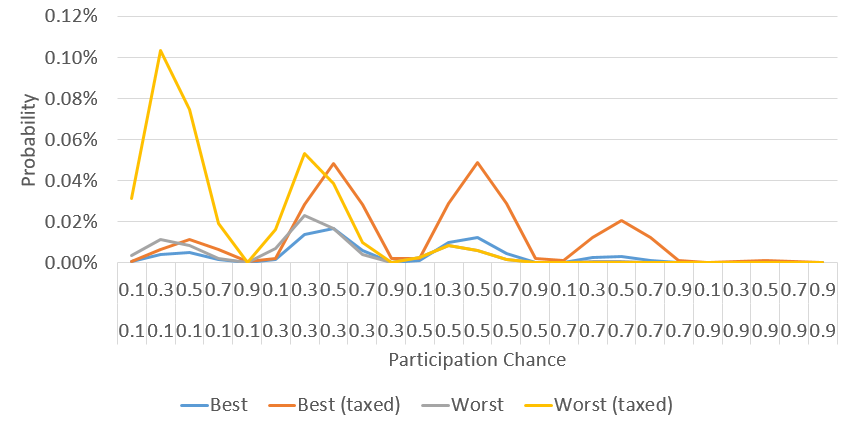
\includegraphics[width=\textwidth]{media/state-bestworst.PNG}
\end{figure}

The peaks in the worst (taxed) trend-line may be due to the low purchase likelihood of the participant directly benefiting the other participant, leading the the largest difference in funds. This was predicted in \cref{table:payout1} in the action combinations (Skip, Purchase). As the purchase probability increases, the peaks reduce in magnitude as probability to reach an equilibrium state increases, decreasing the probability to reach a worst case state. Similarly, the best states are only achievable if neither participant is especially inclined to purchase, increasing the probability of traversing a chain of transitions in which one participant does not purchase chunks, letting the other participant accumulate the rewards unchecked.

Figure \ref{figure:state-expected-tax} below shows the expected reward as tax increases. The test script can be found in \cref{appendix:testparticipationtax} and the raw data can be found in \cref{appendix:state-results-tax} As expected, the reward decreases in a linear fashion as the tax increases.

\begin{figure}[H]
  \centering
  \caption{Expected reward per tax rate}
  \label{figure:state-expected-tax}
  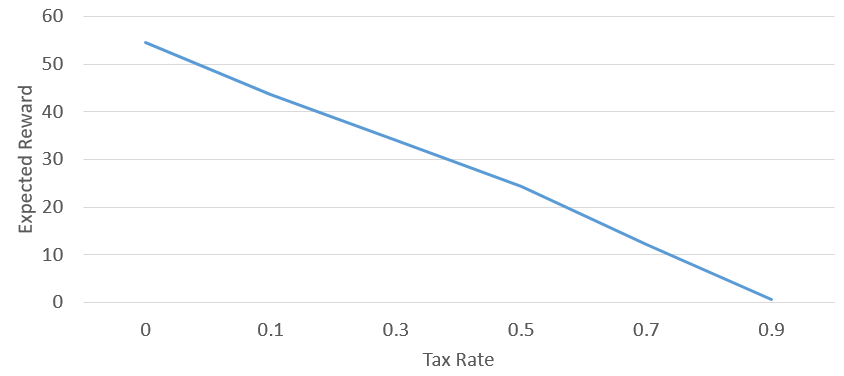
\includegraphics[width=\textwidth]{media/state-expected-tax.PNG}
\end{figure}
